\chapter{Analýza}

\section{Monitorovanie vibrácií a šoku}
Vibrácie sú periodickým kmitaním hmoty okolo rovnovážnej polohy vznikajúce excitáciou látky, ktorej je dodaná potenciálna energia, a zo
zákona zachovania energie je následne premieňaná na kinetickú energiu. V realite dochádza pôsobením trenia k útlmu voľného oscilačného
pohybu s časom  a pohybová energia sa uvoľňuje v podobe tepelnej alebo akustickej emisie do okolitého prostredia. Častejšie ako presné
harmonické kmity sú pozorované náhodné vibrácie, ktorých vývoj nevieme dopredu predvídať. Naproti tomu šok, alebo aj prechodový jav, je
náhle uvoľnenie kinetickej energie krátkeho trvania oproti prirodzenej oscilácii systému.

Význam a dôležitosť sledovania vibrácií spočíva v ich výskyte u každého mechanického zariadenia a je zapríčinená pohybom jednotlivých
súčiastok a trením v ložiskách. Ich nadmerná prítomnosť býva spôsobená opotrebením dielov stroja alebo nevyvážením rotačných častí,
zakliesňovaním ozubených kolies, ako dôsledkoch iných technických defektov. V prevažnej väčšine prípadov ide o nežiaduci jav nakoľko
zakladá zníženiu účinnosti so zvýšením hlučnosti ako vedľajšiemu produktu.

Ďalšou oblasťou hojnej prítomnosti vibrácií je preprava osôb alebo tovaru cestnými a železničnými dopravnými prostriedkami, kde sú
zapríčinené nerovnosťami povrchu vozovky alebo koľaje v bode styku s kolesami vozidla. Na zvýšenie ovládateľnosti vozidla a komfortu
pasažierov sú kabíny odpružené od kolies tlmičmi. Lietadlá sú zasa pod vplyvom trenia vzduchu s trupom a krídlami konštrukcie, ktoré je
ďalej zosilnené vzdušnými prúdmi a turbulenciami.

Druhým významným faktorom podieľajúci sa na tvorbe vibrácii je aparát, ktorý uvádza vozidlo do pohybu alebo zastavuje, čiže hnací
najčastejšie spaľovací, dieselový alebo elektrický motor a brzdový systém. Jedná sa najmä o vplyv pohybu piestov, alebo rotora u
elektrických vozidiel, a prenosu otáčavého pohybu motora cez oje hriadeľa na nápravy. ABS brzdový systém prítomný pri väčšine
automobilov zabraňujú šmyku striedavým zomknutím a uvoľňovaním brzdových kotúčov, čo má tiež vplyv na podmienky počas jazdy.

Detekciou nežiaducich vibrácií v preprave sa dokáže zabezpečiť aj bezpečnosť pasažierov včasnou výmenou súčiastky, ktorá by ovplyvnila
prevádzkyschopnosť v kritických momentoch. Ich eliminácia dokáže predísť nenávratnému poškodeniu krehkých materiálov alebo
znehodnoteniu reaktívnych substancií, či dokonca ich aktivácii v prípade výbušnín a pyrotechniky.

V neposlednom rade sú vibrácie súčasťou potenciálne nebezpečných prírodných úkazov a ich správna identifikácia má za následok varovania
pre preventívnu evakuáciu obyvateľstva v oblasti, ktoré bude zasiahnutá zemetrasením, či erupciou sopky vedúcimi k ohrozenia zdravia
osôb a poškodenia majetku.

\subsection{Meranie fyzikálnej veličiny akcelerácie}
Pohyb mechanického systému vystaveného vonkajším silám sa nazýva odozva, ktorej správanie opisuje zjednodušený model s jedným stupňom
voľnosti (1DOF) kmitajúceho telesa s pružinou a tlmičom \cite{vibrations-shock}.

\begin{figure}[h]
	\centering
	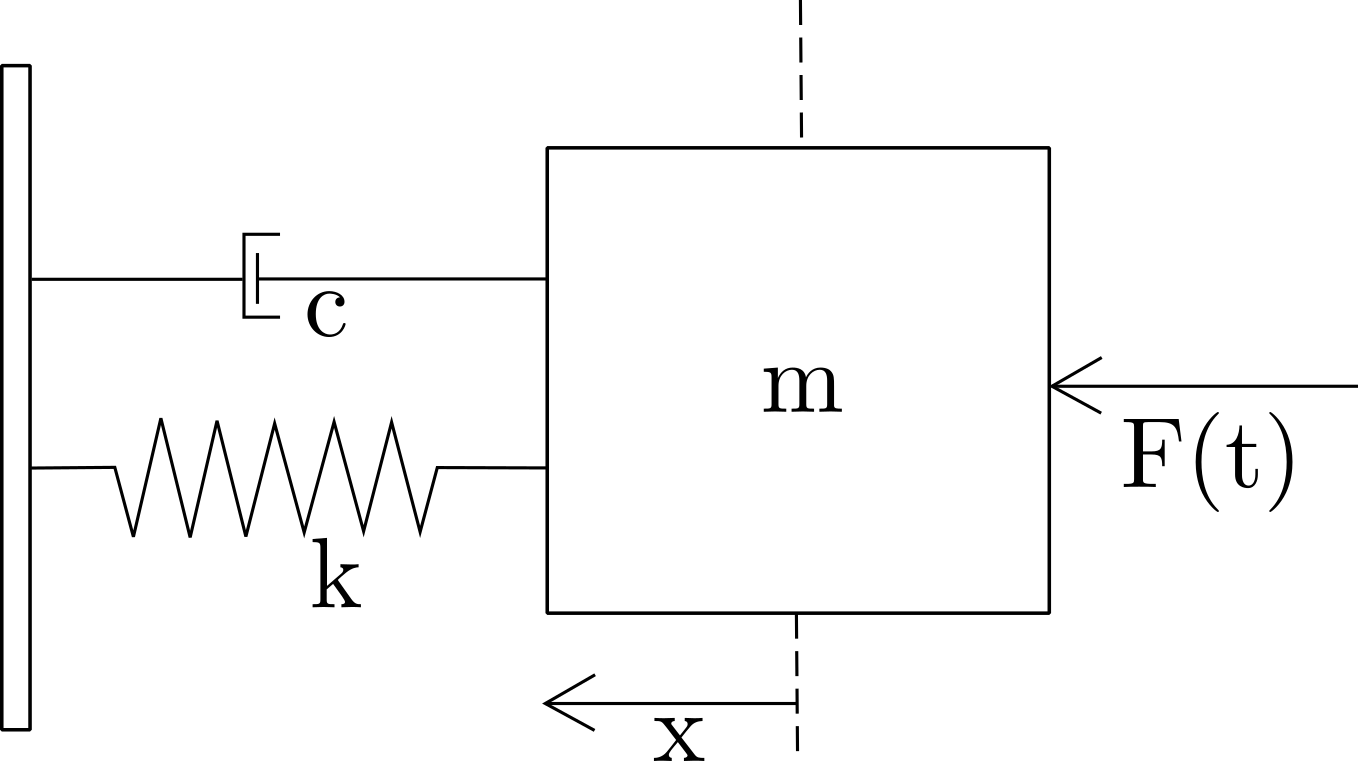
\includegraphics[width=0.7\textwidth]{figures/mass-spring-damper-model.png}
	\caption{Model oscilujúceho systému s pružinou a tlmičom}
\end{figure}

Pri pôsobení vonkajšej sily $F$ na hmotu upevnenú na pružine vznikajú nútené vibrácie, ktoré ju vychyľujú z rovnovážnej polohy. Uvedená sila je charakterizovaná druhým Newtonovým zákonom v tvare $F = ma$, kde $m$ je hmotnosť telesa a $a$ predstavuje zrýchlenie. V protismere pôsobí sila vyvolaná pružinou $F_s = -kx$ a tlmiacim členom $F_d = -cv$, kde $k$ je tuhosť pružiny ovplynená jej konštrukciou, $c$ je tlmiaci koeficient, $x$ je vychýlenie z rovnovážneho stavu, a $v$ rýchlosť vychýlenia. 

Fyzickým obmedzením  telesa, ktorým je viazaný na pevnú podložku dochádza pri zanedbaní deformácie k takmer zaručenému návratu do rovnovážnej polohy a to nám umožňuje merať intenzitu vibrácií cez zrýchlenie ťažidla. Výslednú silu v jednom smere získame sčítaním síl podieľajúcich sa na dynamike telesa.
\begin{ceqn}\begin{align}
 	F(t) = ma - cv - kx
\end{align}\end{ceqn}
Pri použití trojosového akcelerometra, kedy sú evidované všetky tri priestorové súradnice časovo-premennej akcelerácie dostávame
nasledujúcu rovnicu vo vektorovom tvare:
\begin{ceqn}\begin{align}
   \vec{a}(t) = \frac{\vec{F}(t)}{m}
\end{align}\end{ceqn}
Magnitúda akcelerácie s troma súradnicami je daná $L_2$ normou vektora $\vec{a} = (a_x, a_y, a_z)$:
\begin{ceqn}\begin{align}
   |a| = \sqrt{a_x^2 + a_y^2 + a_z^2}
\end{align}\end{ceqn}

\subsection{MEMS kapacitný akcelerometer}
Bežné inerciálne senzory na meranie zrýchlenia priamočiareho, ale aj rotačného pohybu (gyroskop), sa vyrábajú technológiou
\emph{MEMS – mikromechanický systém}, kedy je celé zariadenie vrátane všetkých mechanických súčastí umiestnené na kremík procesom
mikrovýroby vo viacerých vrstvách. Sila spôsobujúca zrýchlenie je potom meraná vychýlením vstavanej odpruženej hmoty vzhľadom
na pevné elektródy, ktoré môžu byť usporiadané jednostranne alebo ako diferenčný pár \cite{mdof-mems-accelerometers}.

\begin{figure}[h]
	\centering
	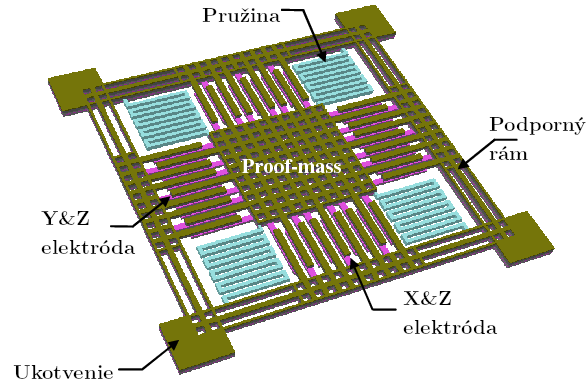
\includegraphics[width=0.8\textwidth]{figures/mems-accelerometer.png}
	\caption{Mikroštruktúra 3DOF MEMS kapacitného akcelerometra \cite{microstructure-mems}}
	\label{fig:mems}
\end{figure}

Pri diferenčnom páre spôsobí pohyb doštičky ťažidla medzi elektródami zmenu kapacít a ich rozdielom je možné zistiť aplikovanú silu a
cez uvedený vzťah zrýchlenie. Na zvýšenie celkovej kapacity sa používa viacero párov elektród zapojených paralelne. Pred prevodom na
číslicový signál musí napäťová úroveň zo senzora prejsť úpravou zahŕňajúcou nábojovocitlivý predzosilňovač, osovú demoduláciu a anti-
aliasingové filtrovanie. 

Viacosové akcelerometre vyžadujú viaceré opísané štruktúry orientované kolmo na seba, podľa obr. \ref{fig:mems}, s ohľadom na počet 
vyžadovaných stupňov voľnosti, pričom v skutočných senzoroch vždy existuje aspoň minimálna závislosť medzi osami rádovo najviac v 
jednotkách percent. Teplota ovplyvňuje citlivosť MEMS akcelerometrov len nepatrne v stotinách percenta na stupeň Celzia.

Akcelerometre sa odlišujú v niekoľkých dôležitých vlastnostiach, ktoré zvyknú byť nastaviteľné vo výrobcom stanovenom rozsahu
prípustných hodnôt s príslušnými toleranciami \cite{accelerometer-mechanics}.

\emph{Citlivosť} stanovuje najmenšiu rozlíšiteľnú zmenu v odčítanom napätí ku zmene externého pohybu respektíve zrýchlenia.
Uvádza sa v jednotkách \emph{mV/g} (milivolt na tiažové zrýchlenie) pri analógovom výstupe, alebo \emph{mg/LSB} (mili-g
na najmenej významový bit). pri senzoroch so vstavaným analógovo-digitálnym prevodníkom. Jednotka \emph{mg/LSB} vyjadruje
o koľko sa zmení zrýchlenie keď zvýšime alebo ponížime binárne číslo na výstupe o jedna. Niekedy sa namiesto
citlivosti uvádza mierka pre presnosť ako prevrátená hodnota citlivosti v \emph{LSB/g}. Tiažové zrýchlenie $g$ sa mierne líši podľa
zemepisnej šírke, ale stanovený prepočet na jednotky SI je $1 g = 9.80665\,m/s^2$
\footnote{\url{https://physics.nist.gov/cgi-bin/cuu/Value?gn|search_for=acceleration}}.

\emph{Dynamický rozsah} sa uvádza v tiažovom  zrýchlení $g$. Hovorí o najmenšej a najväčšej rozlíšiteľnej hodnote zrýchlenia nad
úrovňou ktorej už dochádza k skresleniu signálu orezaním špičiek. S nevyhnutnými drobnými nepresnosťami výroby mikromechaniky je tzv.
\emph{zero-g napätie} popisujúce odchýlku skutočného od ideálneho výstupu, keď na sústavu nepôsobí žiadne zrýchlenie. Za ideálnych
okolností bez pohybu na vodorovnom povrchu namerajú osi $x$ a $y$ zrýchlenie $0g$, zatiaľčo na $z$ pôsobí $1g$. Očakávaním je nulová
hodnota výstupného napätia a tým aj výstupného registra.

\emph{Šírka pásma} senzora v \emph{Hz} predurčuje rozsah frekvencie vibrácií, ktoré je možné zachytiť. Podmienená je zvolenou
početnosťou  čítania akcelerácie za sekundu, čiže vzorkovacou frekvenciou. Stanovuje sa tiež nastaviteľným parameterom \emph{ODR}
(Output Data Rate) - výstupný dátový tok, pričom šírka pásma je spravidla polovicou ODR. Menej uvádzanou vlastnosťou býva 
\emph{frekvenčná odozva} senzora, ktorá určuje o koľko sa v rámci tolerancie odlišuje skutočná 
citlivosť od referenčnej pre zodpovedajúcu frekvenciu vibrácii. 

Na meranie zrýchlenia má nevyhnutný vplyv šum zapríčinený Brownovým  pohybom a nedokonalosťou skutočných materiálov v štruktúre 
akcelerometra. Intenzita šumu rastie inverznou odmocninou so šírkou pásma, čiže s častejším meraním získavame menšiu presnosť. Pri 
dostatočnom odstupe signálu od šumu, $SNR = P_{signal} / P_{šum}$, umožňuje hardvér akcelerometra vzorkovať amplitúdy až nad stanovený 
prah generovaním prerušenia, čím sa dokáže efektívne zbaviť nevýznamných fluktuácií.

\subsection{Analógovo-digitálny prevodník}
Spojitá napäťová úroveň transformuje analógovo-digitálny (A/D) prevodník pre spracovanie digitálnym systémom do množiny diskrétnych
hodnôt. Vstupný signál najprv prechádza fázou vzorkovania, kedy sa vzorky zaznamenávajú v pravidelných intervaloch. Počet vzoriek
odčítaných za sekundu je vyjadrený vzorkovacou frekvenciou $f_s$ v $Hz$. Časový rozdiel medzi vzorkami, nazývaný perióda vzorkovania,
je prevrátenou hodnotou vzorkovacej frekvencie $T_s = \frac{1}{f_s}$. Pre presnú rekonštrukciu pásmovo obmedzeného signálu v hraniciach
$[-f_{max}; f_{max}]$ je nevyhnuté podľa \emph{Nyquist-Shannonovej vety} o vzorkovaní, aby vzorkovacia frekvencia bola najmenej 
dvojnásobkom maximálnej frekvencie snímaného signálu.
\begin{ceqn}\begin{align}
   f_s \geq 2 \cdot f_{max}
\end{align}\end{ceqn}

Každej vzorke je následne v procese kvantovania priradená diskrétna hodnota s konečným počtom $n$ bitov, ktorá je najbližšia možná ku
skutočnej hladine analógového vstupu. Dochádza pritom k istému zaokrúhľovaniu z dôvodu nepresnosti vyjadrenia spojitej domény amplitúd
diskrétnym číslom. Tento jav označujeme ako kvantizačný šum, ktorý je najviac polovicou z maximálnej rozlíšiteľnej zmeny signálu a
trpia nim všetky existujúce A/D prevodníky. Rovnako tak sa u všetkých prevodníkov prejavuje aspoň nepatrná miera nelinearity výstupného
kódu, chýbajúce kódy alebo ich nemonotónnosť.

\begin{figure}[h]
	\centering
	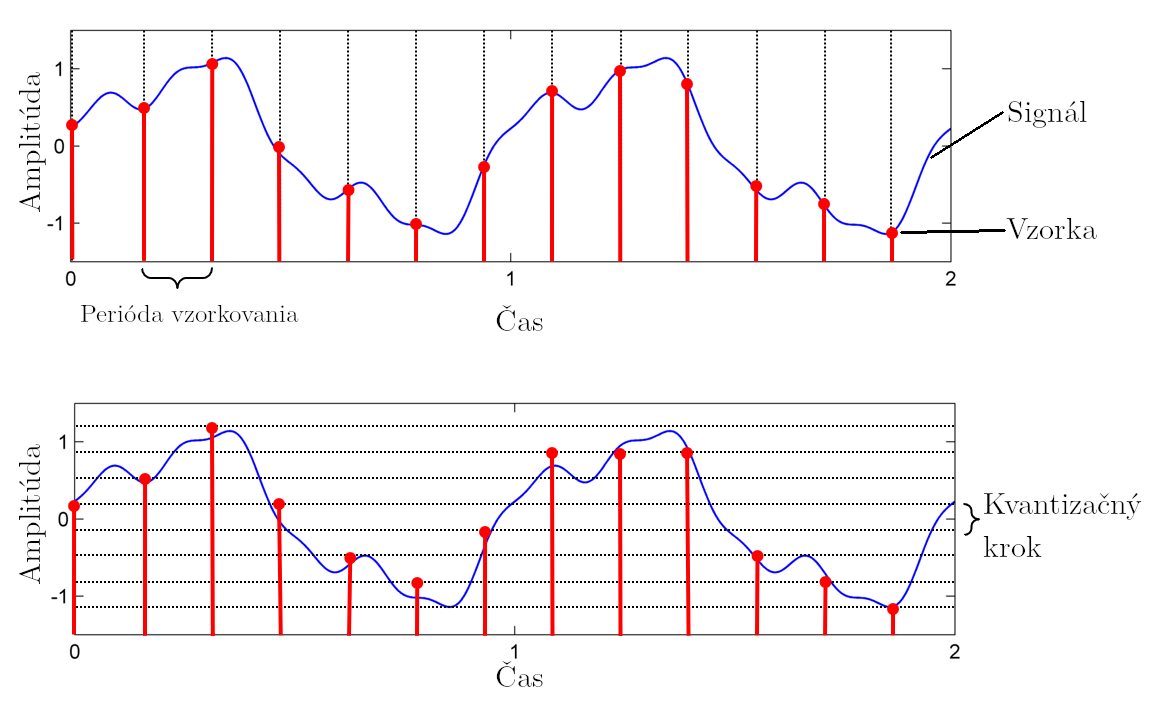
\includegraphics[width=0.8\textwidth]{figures/analog-to-digital-conversion.png}
	\caption{Digitalizácia signálu v analógovo-digitálnom prevodníku \cite{music-processing}}
\end{figure}

Prevodníky integrované priamo s inerciálnymi jednotkami sa vyhotovujú v rozlíšeniach 12, 16 alebo 20 bitov. Umožňujú tak pripojiť
akcelerometer rovno na sérové zbernice \emph{SPI} alebo \emph{I2C}. Všeobecne platí, že pri $n$ bitoch je k dispozícii $2^n$ rozličných
čísel. Kódovaním v dvojkovom doplnku pre zachytenie záporných hodnôt sa uvažuje s intervalom $[-2^\frac{n}{2}; 2^\frac{n}{2} - 1]$.

Napríklad pri 12-bitovom A/D prevodníku s referenčným napätím $3.3V$ je teoreticky najmenšia rozlíšiteľná zmena na najmenej významový
bit $3.3V / 2^{12} = 0.81 mV$. Ak je rozhranie senzora priamo vybavené analógovým výstupom nič nebráni v použití presnejšieho
prevodníka, napriek tomu najmenší merateľný dielik je zdola stále ohraničený citlivosťou akcelerometra.

Číslicovú hodnotu v dvojkovom doplnku získanú konverziou $\hat{x}$ je z dôvodu širšej zrozumiteľnosti žiaduce prepočítať na
štandardné fyzikálne jednotky pre zrýchlenie, $a$ v $m/s^2$). $R$ prestavuje nastavený dynamický rozsah v jednotkách $g$ a $n$
je počet bitov A/D prevodníka.
\begin{ceqn}\begin{align}
   a = \hat{x} \cdot ((R \cdot g) / 2^{n / 2})
\end{align}\end{ceqn}

Na základe už zmieneného ohľadom vlastností MEMS akcelerometrov, presnejší prevod dosiahneme zužitkovaním deklarovanej citlivosti
senzora pri danom dynamickom rozsahu $S_R$ udávaného v $mg/LSB$.
\begin{ceqn}\begin{align}
   a = \hat{x} \cdot (S_R \cdot g) / 1000
\end{align}\end{ceqn}

\subsection{Vlastnosti bežných akcelerometrov}
Na ilustráciu uvádzame parametre zvolených najrozšírenejších typov akcelerometrov. Akcelerometer LSM9DS1 \cite{lsm9ds1} umožňuje cez
zbernicu SPI alebo I2C zvoliť zo štyroch dynamických rozsahov, pričom každé rozpätie sa vyznačuje svojou citlivosťou. Zvolením menšieho
dynamického rozsahu zvýšime citlivosť. LSM9DS1 funguje pri rozsahoch $\pm2$g, $\pm4$g a $\pm8$g a $\pm16$g, postupne s citlivosťami
$0.061$ mg/LSB, $0.122$ mg/LSB, $0.244$ mg/LSB, $0.732$ mg/LSB. Výstupný dátový tok (ODR) je možné nastaviť na $10$Hz, $50$Hz,
$119$Hz, $238$Hz, $476$Hz a najvyššie na $952$ Hz. Navzorkované hodnoty sú ukladané do 16-bitového výstupného registra v
dvojkovom doplnku.

Nízkoenergetický 3DOF MEMS akcelerometer ADXL362 \cite{adxl362} so spotrebou $2\,\mu A$ pri $100$Hz disponuje
rozsahmi $\pm2$g, $\pm4$g a $\pm8$g s citlivosťami $1$, $2$ a $4$ mg/LSB. Dostupné vzorkovacie frekvencie 12-bitového A/D prevodníka sú
$12.5 - 400$Hz v 8 krokoch vždy po násobkoch predošlého kroku. Pre rýchlejšie čítanie pri nižšom rozlíšení dokáže senzor zakódovať dáta
do 8-bitového registra.

Vyrábajú sa tiež akcelerometre s väčšími dynamickými rozsahmi a nízkym šumom, ide napríklad o ADXL356 a ADXL357 \cite{adxl357} so
škálami $\pm 10$g, $\pm 20$g a $\pm 40$g s citlivosťou $0,019$ mg/LSB po $0,078$ mg/LSB a rozlíšením A/D prevodníka 20 bitov pri
ODR $4 - 4000$Hz. ADXL357 ponúka priamo analógové výstupy s citlivosťou $20 - 80$ mV/g pri napájaní $3.3$ V.

\subsection{Odvodzovanie rýchlosti a dráhy zo zrýchlenia}
Meranie akcelerácie umožňuje zároveň nepriamo získať ďalšie údaje o pohybe celkovom v priestore ako aj spôsobenom vibráciami.
Zrýchlenie $\vec{a}$ je definované ako časová zmena rýchlosti $\vec{v}$, zatiaľčo rýchlosť je časovou zmenou polohy $\vec{r}$. Na
pozorovanie prechodových javov alebo na vyjadrenie miery plynulosti pohybu slúži ryv $\vec{j}$, ktorý je časovou zmenou akcelerácie.
Pokiaľ nie sú známe počiatočné podmienky v okamihu začiatku snímania akcelerácie, budú hodnoty veličín relatívne vzhľadom na
štart záznamu. Kinematika v diskrétnom čase je potom opísaná nasledujúci rovnicami, kde $\Delta$ je operátor diferencie
$\Delta t = t(i) - t(i-1)$:

\begin{ceqn}\begin{align}
   \vec{v} = \frac{\Delta \vec{r}}{\Delta t}; \;\;
   \vec{a} = \frac{\Delta \vec{v}}{\Delta t}; \;\;
   \vec{j} = \frac{\Delta \vec{a}}{\Delta t}
\end{align}\end{ceqn}

Vyjadrenie neznámych premenných vzhľadom na akceleráciu spočíva v prenásobení rovníc členom $\Delta t$, čím sa získajú
vzťahy pre okamžitú dráhu a okamžitú rýchlosť. Spočítaním čiastkových okamžitých rýchlostí na intervale dostaneme celkovú rýchlosť a
rovnaký úsudok platí pre polohu. V spojitom čase, keď by vzorkovacia perióda bola nekonečne krátka, dochádza naproti tomu k
integrovaniu funkcie akcelerácie. Dostávame, že rýchlosť je integrálom zrýchlenia a poloha je dvojným integrálom zrýchlenia:

\begin{ceqn}\begin{align}
   \vec{v}(t) = \vec{a_0} + \int{\vec{a}(t)\,\mathrm{dt}} \\
   \vec{r}(t) = \vec{r_0} + \vec{v_0}t + \iint{\vec{a}(t)\,\mathrm{dt}}
\end{align}\end{ceqn}

\subsection{Numerická kvadratúra}
Približný výpočet určitého integrálu funkcie akcelerácie je založený na geometrickej interpretácii integrálu ako plochy pod krivkou.
Hovoríme vtedy o probléme numerickej kvadratúry, ktorý navrhuje nahradiť pôvodný integrand interpolačným polynómom 
\cite{numerical-mathematics}. Rád polynómu $n$ implicitne stanoví priebeh funkcie medzi ekvidištantnými vzorkami a 
má dopad na presnosť aproximácie. Najčastejšie sa používajú konštantný ($n = 0$), lineárny ($n = 1$) alebo kvadratický ($n = 2$) 
polynóm, podľa toho rozlišujeme obdĺžnikové pravidlo (vzorec \ref{eq:midpoint-rule}),
lichobežníkové pravidlo (vzorec \ref{eq:trapezodial-rule}) a Simpsonovo pravidlo (vzorec \ref{eq:simpson-rule}).

\begin{ceqn}
\begin{align}
   v(t_i) &= T_s \cdot a\left(\frac{t_i + t_{i-1}}{2}\right)  \label{eq:midpoint-rule} \\
   v(t_i) &= \frac{T_s}{2} \cdot [a(t_i) + a(t_{i-1})]		\label{eq:trapezodial-rule} \\
   v(t_i) &= \frac{T_s}{3} \cdot [a(t_{2i}) + 4a(t_{2i - 1}) + a(t_{2i - 2})] \label{eq:simpson-rule}
\end{align}
\end{ceqn}

Pri \emph{obdĺžníkovom pravidle} (obr. \ref{fig:midpoint-rule}) nepripúšťame zmenu hodnoty zrýchlenia medzi vzorkami a okamžitú 
rýchlosť, čiže plochu, odhadneme ako dĺžku intervalu vzorkovania vynásobenú priemerom výšok dvoch následných pozorovaní. Interpolačný 
polynóm je konštantná funkcia. \emph{Lichobežníkové pravidlo} (obr. \ref{fig:trapezodial-rule}) uvažuje s lineárnou zmenou veličiny 
medzi meraniami, preto interpoluje priamkou.\emph{Simpsonovo pravidlo} (obr. \ref{fig:simpson-rule}) sa snaží o ešte tesnejší odhad s 
využitím kvadratickej funkcie. Každé kvadratúrne pravidlo sa síce vyznačuje presne vyčísliteľnou chybovosťou, ale k tomu je nevyhnutné 
poznať analytické vyjadrenie vibrácií, čo dáva realistický odhad len pri čisto periodických kmitoch.

\begin{figure}[h]
\centering
\begin{subfigure}[b]{0.32\textwidth}
    \centering
    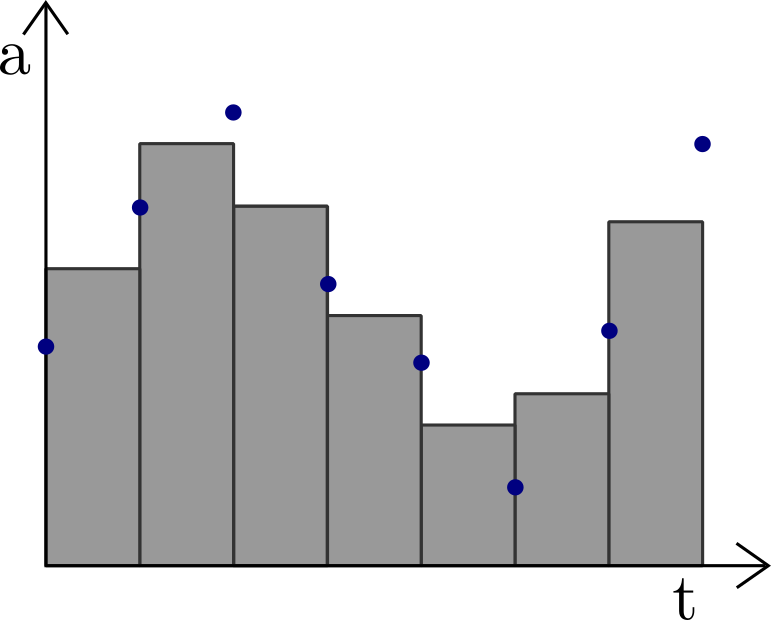
\includegraphics[width=\textwidth]{figures/rectangular-rule.png}
    \caption{Obdĺžníkové}
    \label{fig:midpoint-rule}
\end{subfigure}
\hfill
\begin{subfigure}[b]{0.32\textwidth}
    \centering
    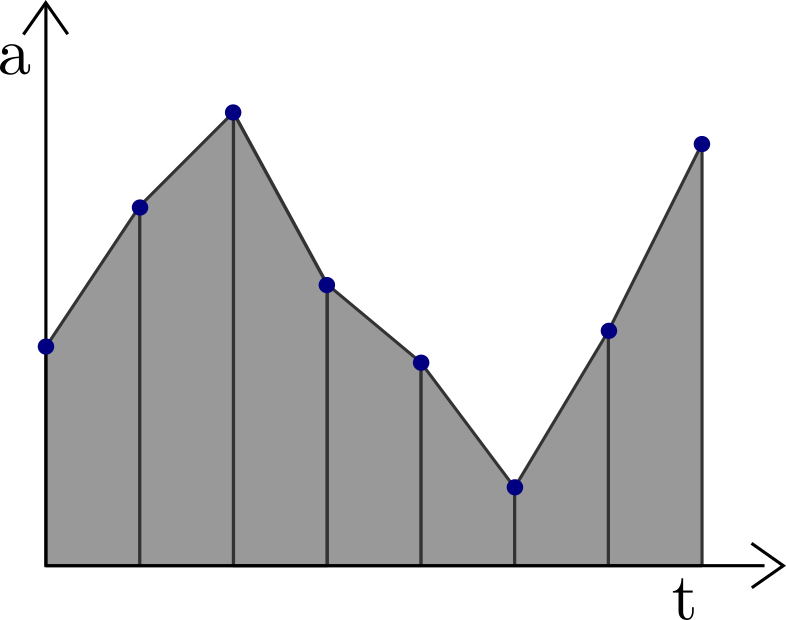
\includegraphics[width=\textwidth]{figures/trapezoidal-rule.png}
    \caption{Lichobežníkové}
    \label{fig:trapezodial-rule}
\end{subfigure}
\hfill
\begin{subfigure}[b]{0.32\textwidth}
    \centering
    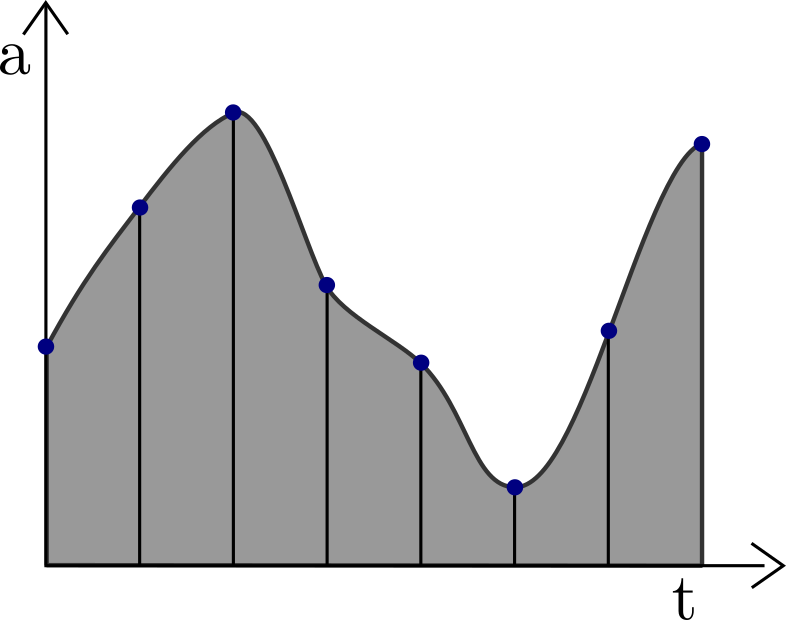
\includegraphics[width=\textwidth]{figures/simpson-rule.png}
    \caption{Simpsonovo}
    \label{fig:simpson-rule}
\end{subfigure}
\caption{Porovnanie pravidiel numerickej integrácie}
\end{figure}

Priama integrácia zašumeného signálu zrýchlenia vedie k neskutočnému driftu, ktorý je ešte zvýraznený dvojitou integráciou pri
odvodzovaní relatívneho posunutia. Dochádza k zosilneniu nízkych a potlačeniu vyšších frekvencií, čím sa začne dominovať neexistujúci
trend vo výstupných dátach. Očakávané oscilujúce správanie vychýlenia u vibrácií so zväčšujúcim sa počtom sčítancov pri rekurentnom
výpočte zaniká. Na zlepšenie stability integrátora sa uplatňuje korekcia cez obálky \cite{integration-acceleration-envelopes}.

Najprv je na vstupnom signále vykonaná zvoleným pravidlom numerická kvadratúra, ktorá môže byť realizovaná na krátkych
úsekoch funkcie, aby sa predišlo pretečeniu pri výraznej akumulácií odklonu. Prichádza k identifikácií lokálnych extrémov, či už maxím,
respektíve miním (pozri \ref{peak-detection}) a ich interpoláciou s kubickou B-spline sa sformuje horná $e_u(t)$, respektíve dolná
obálka signálu $e_d(t)$. Obálky sú spriemerované $\bar{e}(t)$, čím vznikne odhad trendovej krivky, ktorá je od už integrovaného
signálu odčítaná $g(t) = f(t) - \bar{e}(t)$. V prípade výpočtu polohy je možné aplikovať uvedený postup kaskádovito, čiže rovnako
ako akcelerácia je aj signál rýchlosti opäť integrovaný a korigovaný obálkami. Trend je rovnako tak odstrániteľný filtrom na
potlačenie prítomnosti jednosmernej zložky v podobe hornej priepuste (pozri \ref{fir-filter}).

\section{Metódy analýzy signálu v časovej doméne}
Pozorovania veličiny predstavujú udalosti merané sekvenčne v čase, kde je s každou obdržanou hodnotou $x_i$ viazaná unikátna 
časová značka $t_i$. Postupnosť jednotlivých čítaní je jednorozmerný časový rad znázoriteľný ako usporiadaná množina dvojíc pečiatky 
rastúcej v čase a nasnímanej úrovne: $T = \{(t_1, x_1),(t_2, x_2), …, (t_n, x_n)\}$. Vzorkovaním v pravidelných intervaloch stačí 
uvažovať namiesto časových značiek o celočíselných indexoch, ktoré určujú pozíciu prvkov vo vektore pozorovaní: 
$\mathbf{x} = (x_1, x_2, …, x_n)^T$. Keď sú súčasne zaznamenávané viaceré dátové body hovoríme o matici pozorovaní $X_{n,m}$, či o 
viacrozmernom časovom rade.

Pri veľkom objeme prichádzajúcich vzoriek produkované senzormi, nie je uskutočniteľné ich úplné uchovanie ani spracovanie celkého 
dátového toku naraz. Častokrát by stratégia neuváženého odkladania viedla k plýtvaniu zdrojov a zbytočnému archivovaniu údajov s nízkou 
informačnou hodnotou. Vhodnejšie je agregovanie toku údajov podľa preddefinovaného zmysluplného kritéria, ktoré by umožňovalo zachytiť 
významné rysy a prompte zodpovedať na vyžadované dopyty. Napríklad zrýchlenie vozidla v konkrétnom okamihu nebude až tak podstatné v 
porovnaní so znalosťou trvania úsekov pridávania alebo brzdenia, či priemernej prudkosti s akou tieto aktivity boli činené. 

\subsection{Prúdové algoritmy}
Priamočiarou realizáciou agregácie je nahliadať na prvky časového radu postupne ako prichádzajú. 
Prúdové algoritmy pôsobiace v reálnom čase, a teda neschopné vidieť finálny vektor vzoriek vstupu sa vyznačujú vlastnosťou, že 
vyprodukujú len na základe takého čiastkového vstupu parciálny výsledok platný pre dosiaľ sa vyskytnutú podmnožinu. 

Online algoritmus  spracúvajúci neprestajný potenciálne nekonečne sa rozširujúcu vstupnú sadu sa ideálne vyznačuje sublineárnou alebo 
polylogaritmickou časovou zložitosťou spracovanie jednotlivých prvkov, celkové spracovanie, a sú žiaduce sublineárne pamäťové nároky 
\cite{data-streams}. Nie za každej situácie sú však dané nároky z praktických dôvodov naplniteľné, snaha je sa k nim aspoň čo najlepšie 
priblížiť. Bod $x_i$, ktorý je súčasťou prúdu sa pri online agregácii zaráta do každého relevantného počítadla, a môže byť ihneď 
zabudnutý, čo sa označuje ako turniketový, prípadne pokladňový, model. Turniket je všeobecnejší formalizmus ako pokladňa, pretože 
umožňuje prvky z počítadla aj odrátavať \cite{data-streams}.

\subsection{Posuvné a rozširujúce sa okná}
Časový rad $\left(x_i\right)_{i = 0}^{n}$ s dĺžkou $n$ môže byť pre účely výpočtu sumárnych štatistík rozdelený oknovou funkciou 
$\mathcal{W}_{l, d}$ na podpostupnosti nazývané okná. 

\emph{Posuvné okná} (,,rolling window'') majú spravidla konštatnú dĺžku $l$ 
menšiu ako celkovú veľkosť radu a sú aplikované s krokom odstupu $d$ pozorovaní. Rad pozorovaní pozostáva z $ (n - (l  - 1)) / d$ 
okien \cite{online-anomaly-detection}. Prirodzene sa posuvné okná objavujú pri manipulácii s vyrovnávacou pamäťou, ktoré sa využívajú 
pri blokovom prenose z adaptéra senzora do hlavnej pamäte. Vtedy sa veľkosť bloku sa rovná posunu $l = d$.

\emph{Rozširujúce sa okná} (,,expanding window'') nachádzajú uplatnenie v menej prípadoch, spravidla sa jedná o inkrementálny 
odhad globálnej štatistiky, ktorá má zmysel prevažne pri sledovaní stabilného javu. \cite{practical-time-series}. Okno začína na 
stanovenej minimálnej veľkosti a s pribúdajúcim počtom bodov ich zahŕňa, čím sa zväčšuje. Dostavuje sa rovnaký výsledok ako v 
turniketovom modeli, ale navyše neplatí obmedzenie zahadzovania už započítaných údajov, ale dokážeme teoreticky operovať so všetkými 
vzorkami vrámci okna.  

\subsection{Číselné charakteristiky štatistického rozdelenia}
Náhodné vibrácie vyskytujúce sa pri skutočných materiáloch sú stochastický proces, ktorý tvorí sekvencia časovo indexovaných 
náhodných premenných. Časový rad predstavuje realizáciu tohto stochastického procesu $\mathbf{Y} = (X_1, X_2, ..., X_n)^T$, kde $X_t$ 
je náhodná premenná so svojím rozdelením pravdepodobnosti. Všeobecne sa pri ideálnych stacionárnych otrasoch predpokladá, že premenné 
pochádzajú z unimodálnej Gaussovej distribúcie: $X_t \sim N(\mu, \sigma^2)$ \cite{vibrations-shock}. 

Sumárna deskripcia nameraného deja pre extrakciu typických čŕt konkrétnych pozorovaných situácií sa uskutočňuje viacerými štatistikami
$h(X_1, X_2, ..., X_n)$ zostručňujúcimi opis funkcie hustoty rozdelenie. Na rozmiestnenie hodnôt meraní v priebehu časového úseku 
sa nazerá z pohľadu polohy, rozptýlenosti a tvaru. Rozsah oboru hodnôt je amplitúda špička-špička (,,peak-to-peak''), 
ktorá je rozdielom maximálnej a minimálnej úrovne, údaj známy tiež ako variančné rozpätie \cite{zaklady-statistiky}.
\begin{ceqn}\begin{align}
x_{pp} = \max_{t \in \mathcal{W}}\{x_t\} - \min_{t \in \mathcal{W}}\{x_t\}
\end{align}\end{ceqn} 
Priemernú energiu obsiahnutú v signále predstavuje štvorec efektívnej amplitúdy RMS a určí sa ako kvadratický priemer pozorovaní:
\begin{ceqn}\begin{align}
x_{rms} = \sqrt{\frac{1}{n}\sum_{t=1}^{n}{x_t^2}}
\end{align}\end{ceqn}
Mierami polohy rozdelenia pozorovaní sú stredná hodnota, informujúca
o centre hodnôt veličiny, a kvantily rozkladajúce usporiadaný vektor pozorovaní na určený počet rovnakých skupín.
Nevychýleným bodovým odhadom strednej hodnoty je \emph{výberový priemer}, ktorý je zároveň amplitúdou jednosmernej zložky signálu:
\begin{ceqn}\begin{align}
\bar{x} = \frac{1}{n} \sum_{t = 1}^{n}{x_t}
\end{align}\end{ceqn}
Najvýznamnejším kvantilmi sú kvartily $Q_q$ vytvárajúce štyri rovnako veľké časti z pôvodných dát, konkrétne dolný kvartil $Q_1$ 
oddelí  25\% najmenších údajov, medián $Q_2$ predelí zoradené údaje na polovicu a horný kvartil $Q_3$ zahrnie 75\% nižších hodnôt. 
Hľadaný kvartil je $k$-ty najmenší prvok v utriedenom zozname meraní, pričom podľa želaného kvartilu $q$ a počtu pozorovaní je 
$k = \lceil n \cdot (1 / q) \rceil$. 

Zistenie $k$-teho najmenšieho prvku s časovou zložitosťou $\mathcal{O}(n \log n)$ umožňuje ľubovoľný lepší triediaci algoritmus
napríklad triedenie zlučovaním (merge sort). Algoritmus \emph{Quickselect} dokáže taký prvok objaviť v čase $\mathcal{O}(n)$. 
V každom kroku vyberie náhodný deliaci bod (pivot) a preskupí k sebe hodnoty menšie ako pivot naľavo a väčšie ako pivot 
napravo. Najmenší prvok následne hľadá v časti, kde zostalo viac ako $k$ prvkov. Pokiaľ došlo k deleniu zoznamu, že pivot
zaujme presne $k$-tu pozíciu prehľadávanie je ukončené a pivot prehlásený za riešenie. Nesprávnym výberom pivota môže 
v najhoršom prípade dôjsť až k zložitosti $\mathcal{O}(n^2)$, čomu sa predchádza výberom pivota cez medián mediánov.

Sústreďovanie realizácie veličiny, respektíve jej rozptýlenosť okolo strednej hodnoty vieme opísať viacerými štatistikami
ako sú \emph{výberový rozptyl} (\ref{eq:variance}), ktorej odmocninou dostaneme smerodajnú odchýlku, 
\emph{priemerná absolútna odchýlka} (\ref{eq:aad}), \emph{mediánová absolútna odchýlka} (\ref{eq:mad})
a \emph{medzikvartilové rozpätie} (\ref{eq:iqr}) \cite{zaklady-statistiky}. Priemerná absolútna odchýlka je 
upraviteľné o mieru centrálnej tendencie, ktorou okrem priemeru môže byť aj medián alebo modus. Vyvarovanie sa 
príliš extrémnym a vychýlením hodnotám docielime zapojením práve mediánu do štatistík absolútnej odchýlky, rovnako
tak to dosiahneme medzikvartilovým rozpätím obmedzením sa na 50\% centrálnych dát.
\begin{ceqn}\begin{align}
	s^2 &= \frac{1}{n - 1} \sum_{t = 1}^{n}{(x_t - \bar{x})^2} \label{eq:variance} \\
	d &= \frac{1}{n} \sum_{t = 1}^{n}(|x_t - \bar{x}|) \label{eq:aad} \\
	\mathrm{MAD} &= med(|x_t - med(\mathbf{x})|) \label{eq:mad} \\
	IQR &= Q_3 - Q_1 \label{eq:iqr}
\end{align}\end{ceqn}

Numericky stabilné bežiace štatistiky priemeru a smerodajnej odchýlky sa udržiavajú cez rekurentné rovnice
\emph{Welfordovho algoritmu} \cite{knuth}. $M_1$ je aktuálna priemerná hodnota údajov v toku a $S_1$ je počítadlo pre
rozptyl, z ktorého je v ktoromkoľvek okamihu získateľná smerodajná odchýlka súboru $\sigma$:
\begin{ceqn}\begin{align}
   M_1 &= x_1;\quad M_k = M_{k-1} + \frac{(x_n - M_{k-1})}{k} \\
   S_1 &= 0; \quad S_k = S_{k-1} + (x_k + M_{k-1})(x_k + M_k)  \\
   \sigma &= \sqrt{S_n / (n - 1)}
\end{align}\end{ceqn}

Tvar distribúcie náhodnej premennej opisujú centrálne momenty šikmosť a špicatosť. Šikmosť $\gamma_1 = \mu^3 / \sigma^3$ udáva skosenie 
rozdelenia, pričom platí že záporná šikmosť značí dlhší ľavý chvost a modus funkcie hustoty sa prevažuje napravo. Zatiaľ čo u kladnej 
šikmosti je to naopak (obr. \ref{fig:skewness}). 

Špicatosť $\gamma_2 = \mu^4 / \sigma^4 - 3$ (obr. \ref{fig:kurtosis}) porovnáva rozdelenie pozorovaní so strmosťou krivky normálneho rozdelenia, čiže viacej realizácií leží bližšie alebo ďalej od strednej hodnosti. Kladná špicatosť signalizuje strmejšiu 
a záporná zasa sploštenejšiu distribúciu. Platí, že $\mu_n $ je priemerom hodnôt $(x_t - \bar{x})^n$.
\begin{figure}[h]
\centering
\begin{subfigure}[b]{0.48\textwidth}
    \centering
    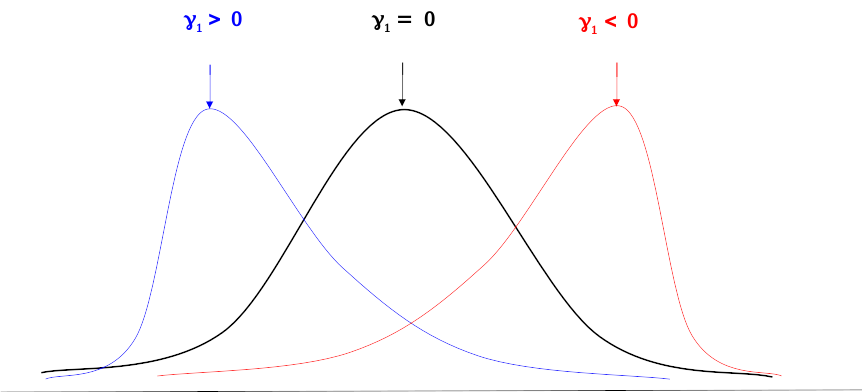
\includegraphics[width=\textwidth]{figures/skewness.png}
    \caption{Šikmosť}
    \label{fig:skewness}
\end{subfigure}
\hfill
\begin{subfigure}[b]{0.48\textwidth}
    \centering
    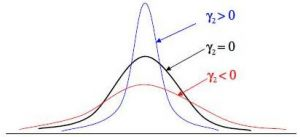
\includegraphics[width=\textwidth]{figures/kurtosis.png}
    \caption{Špicatosť}
    \label{fig:kurtosis}
\end{subfigure}
\caption{Dopad šikmosti a špicatosti na histogram distribúcie}
\end{figure}

Závislosť dvojíc veličín sa vyjadruje \emph{kovariancia} $cov(\mathbf{x}, \mathbf{y})$ a \emph{korelácia} 
$\rho(\mathbf{x}, \mathbf{y})$. U vektora akcelerácie nás bude napríklad zaujímať vzájomná korelácia medzi 
osami pohybu: $\rho(\vec{x},\vec{y}),\, \rho(\vec{x},\vec{z}),\, \rho(\vec{y},\vec{z})$ upozorňujúca na diagonálny 
pohyb alebo podobné budenie v oboch korelovaných smeroch a tým umožňujúce redukciu údajov z dôvodu redundancie.
Kovariancia je daná strednou hodnotou súčinu odchýlky od priemeru zodpovedajúcej premennej (vzťah \ref{eq:covariance}). 
Normovaním kovariancie smerodajnými odchýlkami veličín získame \emph{Pearsonov korelačný koeficient}
(vzťah \ref{eq:correlation}), ktorý je z intervalu $[-1; 1]$.  Hodnota koeficientu $-1$ značí nepriamu lineárnu závislosť
a $+1$ priamu závislosť. 
\begin{ceqn}\begin{align}
\mathrm{cov}(\mathbf{x}, \mathbf{y}) &= \frac{1}{n} \sum_{t=1}^{n}{(x_t - \bar{x})(y_t - \bar{y})} \label{eq:covariance} \\
\rho(\mathbf{x}, \mathbf{y}) &= \frac{\mathrm{cov}(\mathbf{x}, \mathbf{y})}{\sigma_x \sigma_y} \label{eq:correlation}
\end{align}\end{ceqn}

\subsection{Algoritmy na rozpoznávanie špičiek}
\label{peak-detection}
lokálne minimá a maximá extrémy - cez prvú a druhú deriváciu, 
\cite{survey-peaks-valleys}
$x_0 \in I$
lokálne maximum $f(x_0) \geq f(x), \forall x \in I$ 
lokálne minimum  $f(x_0) \leq f(x), \forall x \in I$
globálne ak interval predstavuje celý definičný obor funkcie

topografická prominencia a izolácia - relatívna výška vrchola / extrému

vyhladzovanie: mean filter, derivative filter (diskrétny derivačný operátor) - sobel filter, Savitzky–Golay filter
\cite{spectrometry-peak-detection}

Vzájomná korelácia - jadra vrchola a signálu
detect peaks in a signal and to measure their positions, heights, widths, and/or areas


\subsubsection{Detekcia prahom pri periodických javoch}
Nad + pod konštantný prah y < t, y > t
x má väčšiu šancu byť nad ako pod priemerom

\begin{ceqn}\begin{align}
y = max\{x_t\} \\
x > \bar{x} \\
t\ =\frac{\frac{u\ \ +\ d}{2}+u}{2} \\
|x - \hat{x}| \geq \theta \\
z = \frac{|x - \mu|}{\sigma} \approx \frac{|x - \bar{x}|}{S}
\end{align}\end{ceqn}

\subsubsection{Význačnosť vrchola spomedzi susedov}
Preskočí špičky s absolútnou magnitúdou menšou ako \verb|height|. Vo vnútornom cykle zisťuje či je bod vyššie ako všetkých `k` susedov doprava a doľava s toleranciou \verb|epsilon|.

\begin{equation}
\forall c \in \{y_{i-k}, ... y_{i+k}\} - \{y_i\}; \; y_i - c \geq -\epsilon
\end{equation}
\cite{survey-peaks-valleys} 
\begin{ceqn}\begin{align}
x_{i-1} < x_i > x_{i+1}, \forall i = 2, 3, ..., n - 1 \\
x_1 > x_2, x_n > x_{n-1}
\end{align}\end{ceqn}
\url{https://terpconnect.umd.edu/~toh/spectrum/PeakFindingandMeasurement.htm}

\begin{algorithm}
\caption{Najvyšší spomedzi susedov}
\begin{algorithmic}[1]
\Function{Find\_Peaks}{$\vec{y}$, $k$, $\epsilon$, $h$}
	\State $peaks \gets []$ 	\Comment{Množina indexov nájdených špičiek v signále $y$}
	\For{$i \gets k$ \textbf{to} $length(y) - k$}
		\If {$h \neq null$ \textbf{and} $|y[i]| < h$}  \Comment{Ignoruj príliš nízke magnitúdy}
			\State \textbf{continue}
		\EndIf
		\State $possible\_peak \gets true$
		\For{$j \gets -k$ \textbf{to} $k$}
			\If {$b \neq 0$ \textbf{and} $y[i + j] - y[i] > \epsilon$}
				\State $possible\_peak \gets false$     \Comment{Vrchol nemá postačujúcu prominenciu}
			\EndIf
		\EndFor
		\If {$possible\_peak = true$}
			\State $peaks \gets peaks + [j]$
		\EndIf
	\EndFor
	\State \Return $peaks$
\EndFunction
\end{algorithmic}
\end{algorithm}

\subsubsection{Algoritmus prechodu nulou do záporu}
Nájdi vo $n$-krát vyhladenom signále body, že platí: $f'(x) = 0$, kde $f''(x) < 0$ a $|f''(x)| > \theta$. Pre odstránenie hraničných efektov použiť mód 'valid' s prísušným posunom hraníc polí.

Diskrétna verzia:
$$f'(x) = 0 \; \mathrm{(Dotyčnica)} \implies |y_{i+k} - y_{i-k}| \leq \epsilon \;\mathrm{(Sečnica)}$$
$$f''(x) < 0 \implies (y_{i+k} - y_i) - (y_i - y_{i-k}) < 0$$
$$|f''(x)| > \theta \implies |(y_{i+k} - y_i) - (y_i - y_{i-k})| > \theta$$

Parametre:
\begin{itemize}
\item $\epsilon$: tolerancia pre nulovú deriváciu
\item $\theta$: strmosť druhej derivácie, čiže špicatosť vrchola
\item $k$: polovica dĺžka sečnice pre výpočet prvej derivácie
\item $n$: veľkosť konvolučného jadra
\item $smooth$: počet vyhladzovaní
\end{itemize}

\begin{algorithm}
\caption{Prechod druhej derivácie nulou do záporu}
\begin{algorithmic}[1]
\Function{Find\_Peaks\_Zero\_Crossing}{$\vec{y}$, $k$, $\epsilon$, $slope$}
	\State $peaks \gets []$
	\For{$i \gets k$ \textbf{to} $length(y) - k$}
		\If {($|y[i+k] - y[i-k]| \leq \epsilon$ \textbf{and} 
		     \State $(y[i+k] - y[i]) - (y[i] - y[i-k]) < 0$ \textbf{and}
		     \State $|(y[i+k] - y[i]) - (y[i] - y[i-k])| > slope$)}
		    \State $peaks \gets peaks + [i]$
		
		\EndIf
	\EndFor
	\State \Return $peaks$
\EndFunction
\end{algorithmic}
\end{algorithm}

\subsubsection{Algoritmus horského turistu}
Obsahuje pamäťový efekt pre dočasné zmeny a berie ich do úvahy ak lokálne záchvevy prekročia tolerovanú úroveň. Ak sa zmení 'slope' oproti predošlému kroku DeltaY, tak hneď neoznačí za zmenu medzi dolinou a vrcholom, ale až po prekročení nastavených prahov. Skutočnosť z reality: jama != údolie 
\cite{peek-mountaineer-method}

\begin{algorithm}
\caption{Zjednodušený algoritmus horského turistu}
\begin{algorithmic}[1]
\Function{Find\_Peaks\_Hill\_Walker}{$\vec{y}$, $tolerance$, $hole$, $prominence$}
	\State $peaks \gets []$
	\State $i\_change \gets 0$
	\State $y\_valley \gets 0$
	\State $possible\_change \gets false$
	\State $uphill \gets (y[1] - y[0]) \geq 0$
	
	\For{$i \gets 1$ \textbf{to} $length(y)$}
		\State $y\_step \gets y[i] - y[i-1]$
        \State $slope \gets y\_step \geq 0$

        \If {$possible\_change = false$ \textbf{and} $uphill \neq slope$}
        	\State $possible\_change \gets true$   \Comment{Označenie potenciálneho extrému}
        	\State $i\_change \gets i - 1$
        \ElsIf {$possible\_change = true$ \textbf{and} $uphill = slope$}
        	\State $possible\_change \gets false$  \Comment{Potenciálny extrém bol zachvením}
        \EndIf
        
        \If {($possible\_change = true$
        	\State \textbf{and} $uphill \neq slope$
        	\State \textbf{and} $|i - i\_change| > hole$
        	\State \textbf{and} $|y[i] - y[i\_change]| > tolerance$)}

        	\State $posible\_change \gets False$
        	\State $prev\_uphill \gets uphill$
        	\State $uphill \gets slope$
        	\Comment{Významný lokálny extrém potvrdený}
        	
        	\If {$prev\_uphill = false$ \textbf{and} $uphill = true$}
				\State $y\_valley \gets y[i\_change]$   \Comment{Nájdené údolie}
                
            \ElsIf {($prev\_uphill = true$ 
            		\State \textbf{and} $uphill = false$
            		\State \textbf{and}  $|y[i - hole] - y\_valley| > prominence$)}
				\State $y\_peak \gets y[i\_change]$    \Comment{Skutočný vrchol identifikovaný}
				\State $peaks \gets peaks + [i_change]$              
            \EndIf      	
        \EndIf       
	\EndFor
	\State \Return $peaks$
\EndFunction
\end{algorithmic}
\end{algorithm}

\subsubsection{Automatický viacúrovňový detektor špičiek v kvázi-periodickom signále}
Uniformne vzorkovaný signál pozostávajúci z komponentu periodických a kvázi-periodických špičiek. 
Stĺpcová smerodajná odchýlka upravenej matice, špička je pri nulovej sigme. \cite{ampd-algorithm}

\begin{algorithm}
\caption{AMPD algoritmus}
\begin{algorithmic}[1]
\Function{Find\_Peaks\_AMPD}{$\vec{y}$}
	\State $peaks \gets []$
	\State $N = length(y)$	
	\State $L = \lceil N / 2 \rceil - 1$
	
	\For{$k \gets 1$ \textbf{to} $L$}  \Comment{Local maxima scalogram (LMS) $\mathbf{M}[L][N]$}
		\For{$i \gets k + 1$ \textbf{to} $N - k$}
			\If {$y[i-k] < y[i] > y[i+k]$}
				\State $M[k][i] = 0$
			\Else
				\State $M[k][i] = 1$
			\EndIf
		\EndFor
	\EndFor

	\For{$k \gets 1$ \textbf{to} $L$}  \Comment{Súčet matice naprieč riadkami}
		\State $\gamma[k] \gets \sum_{i = 1}^{N}{M[k][i]}$
	\EndFor	
	
	\State $\lambda \gets \mathrm{argmin}(\gamma[k])$ \Comment{Škála $k$ s najväčším počtom lokálnych maxím}
	
	\Comment{Odstránenie riadkov so z $\mathbf{M}$ škálou väčšou ako $\lambda$ na rozmer $\lambda \times N$}
	\For{$i \gets 1$ \textbf{to} $N$}
		\State $\mu_i \gets 1/\lambda \cdot \sum_{k = 1}^{\lambda}{M[k][i]}$  \Comment{Smerodajná odchýlka naprieč škálami}
		\State $\sigma_i \gets 1 / (\lambda - 1) \cdot \sum_{k = 1}^{\lambda}(M[k][i] - \mu_i)^2$
		\If {$\sigma_i = 0$} 
			\State $peaks \gets peaks + [i]$
		\EndIf
	\EndFor
	
	\State \Return $peaks$
\EndFunction
\end{algorithmic}
\end{algorithm}

\subsection{Metriky pre binárny klasifikátor}
Skutočne pozitívny a negatívny $TP$ (hit), $TN$ (miss) - výsledok zodpovedaná značke z anotovaného datasetu skučnému výsledku
Falošne pozívny $FP$ (chyba I. rádu) - proces je normálny, ale registrujeme neočakávané správanie,
Falošne negatívny $FN$ (chyba II. rádu) - proces je abnormálny, ale správanie prechádza bez povšimnutia
Matica zámen 
\begin{table}[]
\begin{tabular}{|l|l|l|}
\hline
             & s Špička & s Nie špička \\ \hline
k Špička     & TP       & FP           \\ \hline
k Nie špička & FN       & TN           \\ \hline
\end{tabular}
\end{table}

Senzitivita, Recall, - tie ktoré NIE SÚ prehlásené za špičky určite NIE SÚ špičky, čo najväčší (nájdené)
$$ TPR = \frac{TP}{P} = \frac{TP}{TP + FN} $$

Chybovosť - čo najmenší
$$  FPR = \frac{FP}{FP + TN}$$

Špecifita - tie ktoré SÚ prehlásené za špičky určite nie SÚ špičky
$$ TNR = \frac{TN}{N} = \frac{TN}{TN + FP} $$

Presnosť - Precision
$$ PPV = \frac{TP}{TP + FP} $$

Accuracy (Presnosť) - koľko zo všetkých identifikuje správne
$$ ACC = \frac{TP + TN}{P + N} = \frac{TP + TN}{TP + TN + FP + FN} $$

F-score - harmonický priemer precision a recall
$$ F_1 = 2 \cdot \frac{PPV \cdot TPR}{PPV + TPR}$$

ROC - kvalita binárneho klasifikátora v závislosi od prahu, 

AUC - x (FPR) ku y (TRP) s rôznym prahom
\cite{anomaly-detection-algorithms}
\cite{wsn-outlier-detection-survey}

\section{Frekvenčná a časovo-frekvenčná analýza signálu}
\cite{time-series-analysis}
vlastnosti frekvenčného spektra,
decibele, 
spektrogram,
odstup od šumu (SNR),
power spectrum density (dbFS),
spektrálny analyzátor

\subsection{Fourierová transformácia}
Diskrétna fourierová transformácia mapuje signál dĺžky $N$ do množiny $N$ diskrétnych frekvenčných komponentov. \cite{signal-processing}
\begin{equation}
X = \mathbf{W}x; W_{nk} = e^{-i\frac{2\pi}{N}nk} = W_N^{nk}
\end{equation}
Inverzná transformácia
\begin{equation}
x = \frac{1}{N}\mathbf{W}^H X
\end{equation}

Integrálne transformácie: Fourierová transformácia (CFT, DFT), Kosínusová transfomácia (MDCT), Vlnková transformácia (CWT) \cite{dct} \cite{casove-frekvencia-analyza-signalu}

\begin{equation}
T(n) = \int{f(t) K(t,x) \mathrm{dt}}
\end{equation}

\begin{equation}
\mathcal{F}: X(\omega) = \int_{-\infty}^{+\infty}{x(t) \cdot e^{-i\omega t} \mathrm{dt}}
\end{equation}

\subsection{Algoritmus FFT pre DFT a DCT}
Opis DIT radix-2 FFT algoritmus komplexných, reálny, pre MDCT \cite{fft-blackbox}

\begin{equation}
X(m) = \sum_{n = 0}^{N-1}{x(n) \cdot e^{-i2\pi n m / N}}
\end{equation}

Frekvenčné rozlíšenie
\begin{equation}
\Delta f = \frac{f_s}{N}
\end{equation}

\subsection{Oknové funkcie}
Gaborová transformácia, Prehľad okien a ich transformácií (sinc), Efekt oknových funkcií na spectral leakage, výhodné percentá prekryvu FT 	\cite{understanding-dsp} \cite{spectral-density-estimation}
Priemerovanie a prekryv - Amplitude Flatness (AF), Power Flatness (PF), Overlap Correlation (OC)

\subsection{Filtre s konečnou impulznou odozvou}
\label{fir-filter}
Roziel medzi FIR a IIR, Dolná pripusť, pásmová priepusť, horná pripusť,
 Konvolúcia a konvolučné jadro, konvolučná veta, účel: identifikácia prítomnosti známej frekvencie v signále akcelerácie
\begin{equation}
y(n) = \sum_{k=0}^{D_y}{x(k) \cdot h(n-k)} = x(n) * h(n)
\end{equation}

Prenosová funkcia
\begin{equation}
H(\Omega) = \frac{Y(\Omega)}{X(\Omega)}
\end{equation}

\subsubsection{Detektor obálok}
\footnote{\url{https://www.mathworks.com/help/dsp/ug/envelope-detection.html}}
\footnote{\url{https://www.dsprelated.com/showarticle/938.php}}

\section{Senzorová sieť}
Nízko-energetické zariadenia komunikujúce cez odľahčené sieťové protokoly so snahou spracovania v reálnom čase a ponechaním najdôležitejších informácii dolovaním z veľkého množstva zdrojových dát. Cloud / Fog comuting. Sink a Edge nodes

Vlastnosti senzorovej siete
\begin{itemize}
\itemsep0em
\item Autokonfigurácia senzora - reakcia na zmeny v sieti a prostredia pôsobenia
\item Škálovateľnosť - veľké množstvo senzorov so spoločným účelom a schopnosťou vzájomnej kooperácie a interoperability.
\item Odolnosť voči chybám - v prípade pridania alebo odobratia uzla budú spojenia bez prerušenia.
\item Energeticky efektívna komunikácia uzlov - s upravenými protokolmi štandardného sieťového zásobníka
\begin{itemize}
\itemsep0em
\item Event-driven - stály zber dát a reakcia na náhle zmeny. posielajú údaje až po prekročený kritického prahu
\item Query-driven - zbierajú údaje iba po prijatí dopytu od používateľa
\item Time-driven - pravidelne odosielajú údaje sinku. vzorkovaciu frekvenciu volí sink
\end{itemize}
\end{itemize}
\cite{wsn-overview}

Spracovanie toku informácií (IFP - Information flow processing) - nástroj na včasné spracovanie dát ako tečie z periférií do centra systému. Snahou je ukladanie agregovaných štatistík, napr. detektor požiaru za použitia čidiel teploty a dymu nepotrebuje ukladať jednotlivé merania, lebo sú samo o sebe nepodstatné. Keď nastane varovná situácia, je potrebné aby tá obsahoval všetky údaje na lokalizáciu ohniska.

CEP - Complex event processing - spracúva toky udalosti zo zdrojov reálneho sveta na základe aplikovania aktívnych pravidiel stanovených správcami systému a poupraví toky do komplexnejšieho výstupu. Pravidlá sú v tvare Event-Condition-Action (ECA).
\begin{itemize}
\itemsep0em
\item Udalosť - definuje zdroje ako generátory udalostí
\item Podmienka - uvažuje ktorá časť udalosti bude braná do úvahy pri spracovaní, napr. môže ísť o prekročenie prahu
\item Akcia - aká sada úloh má byť vykonaná pri detekcii udalosti
\end{itemize}

Behové pravidlá sú spracúvané vo viacerých fázach
\begin{itemize}
\item Signalizácia - detekcia udalosti
\item Spustenie - asociácia udalosti so sadou pravidiel
\item Vyhodnotenie - vyhodnotenie podmienky
\item Plánovanie - stanovenie poradia vykonania
\item Vykonanie - vykonanie pravidlá
\end{itemize}
\cite{processing-information-flows}

\subsection{Senzorová jednotka}

Súčasti senzorovej jednotky:
\begin{itemize}
\item Zberná jednotka
\item Výpočtová jednotka
\item Komunikačná jednotka
\item Napájacia jednotka
\end{itemize}

Obmedzenia na senzorové uzly
\begin{itemize}
\item Spotreba energie - energetická autonómia uzlov vo WSN umožňuje nasadzovanie zariadení do odľahlých miest pre využitie v inteligentných mestách alebo na účely ochrany prírody. životnosť senzorovej jednotky je ohraničená kapacitou batérie.
\item Dosah komunikácie - Senzory disponujú obmedzenou energiou na vysielanie a dosah je negatívne ovplyvnený silou signálu na anténe. Z toho vyplývajú aj nižšie prenosové rýchlosti.
\item Výpočtový výkon a úložisko - Nízka taktovacia frekvencia procesora v megaherzoch a veľkosti pracovných pamätí v stovkách kilobajoch alebo megabajtoch.
\end{itemize}
\cite{big-data-collection-wsn}


Za ideálnych okolností by sa mal online algoritmus učiť kontinuálne bez ukladania predošlých bodov a detekcií.
V rozhodnutiach algoritmu sú zahrnuté informácie o všetkých predošlých bodoch do terajšieho rozhodnutia. Mal by mať schopnosť sa adaptovať dynamickému prostrediu, v ktorom pôsobí. Bez nutnosti manuálnych úprav parametrov modelu. Zároveň je žiaduce minimalizovať falošné pozitíva a negatíva pri detekcii udalostí.


\emptypage
